\documentclass{article} 

\usepackage{algorithmic}
\usepackage[small,bf]{caption}
\usepackage{float}
\usepackage{graphicx}

\graphicspath{{../}}

\floatstyle{plain}
\newfloat{program}{thp}{lop}
\floatname{program}{code}


\begin{document}
    
\title{Stock Exchange Server Simulator}
\author{Anton Morozov and Shubham Chopra}
\maketitle
    
\section{Introduction.}

Our goal is to create a unified format for specifying simulations from historical data. In many instances it is hard, expensive or downright impossible to re-run an experiment. This leads to creating simulations for emulating such experiments under various conditions. During a simulation original data parameters are augmented with new data. A set of user defined rules specify how historical and new data interact. Below we describe a format that allows to freely augment and combine existent data with new data. 

%In these simulations parameters during the progress of an experiment are preserved and we want to either change or augment those parameters with new information. Also we want to let users specify the results of the augmentation. 

\section{Approach.}

At a high level historical data together with new data can be thought of as a stream of updates to a relational table. We assume that there are $N$ update streams, each resulting in its own relational table. These relations can be combined into a set of $K$ additional relations. For each $k$ in $K$ we can describe desired simulation outcomes. The resultant $K$ streams can then be combined, filtered and output as desired.


%parameters for the experiments can be though of as a stream of updates to a relational table.  New data can be thought of as updates to some relation. If we have $N$ update streams, we will end up with $N$ different relations. These relations can be combined into a set of $K$ additional relations. For each $k$ in $K$ we can describe desired simulation outcomes. The resultant $K$ streams can then be combined and filtered and outputted as desired. 

The stock exchange simulator can be thought of as a stream processor. We can assume that there are $N$ streams coming in. Each of these streams is filtered according to certain conditions and merged together if needed. The merged streams form $K$ order-book DBs. These $K$ DBs are fed to a matching engine, which generates a set of output streams.

Generalized specification process for creating a simulator can be described in five steps:

\begin{enumerate}
    \item {\bf Input Filter}: Each input stream can be filtered. This means that each incoming tuple in the stream can either be removed or it can generate extra inputs. 
    \item {\bf Input Merging}: The set of input stream relations can be combined or subdivided into another set of $K$ relations using merging and filtering. 
    \item {\bf Experiment}: For each relation produced at a merging stage is reduced/matched using specifications given by a user.
    \item {\bf Output Merging}: Experiment outcomes can again be combined or filtered.
    \item {\bf Output Filter}: For each output stream additional conditions can be imposed. Data within a stream can be changed based on those conditions.
\end{enumerate}

\begin{figure}
  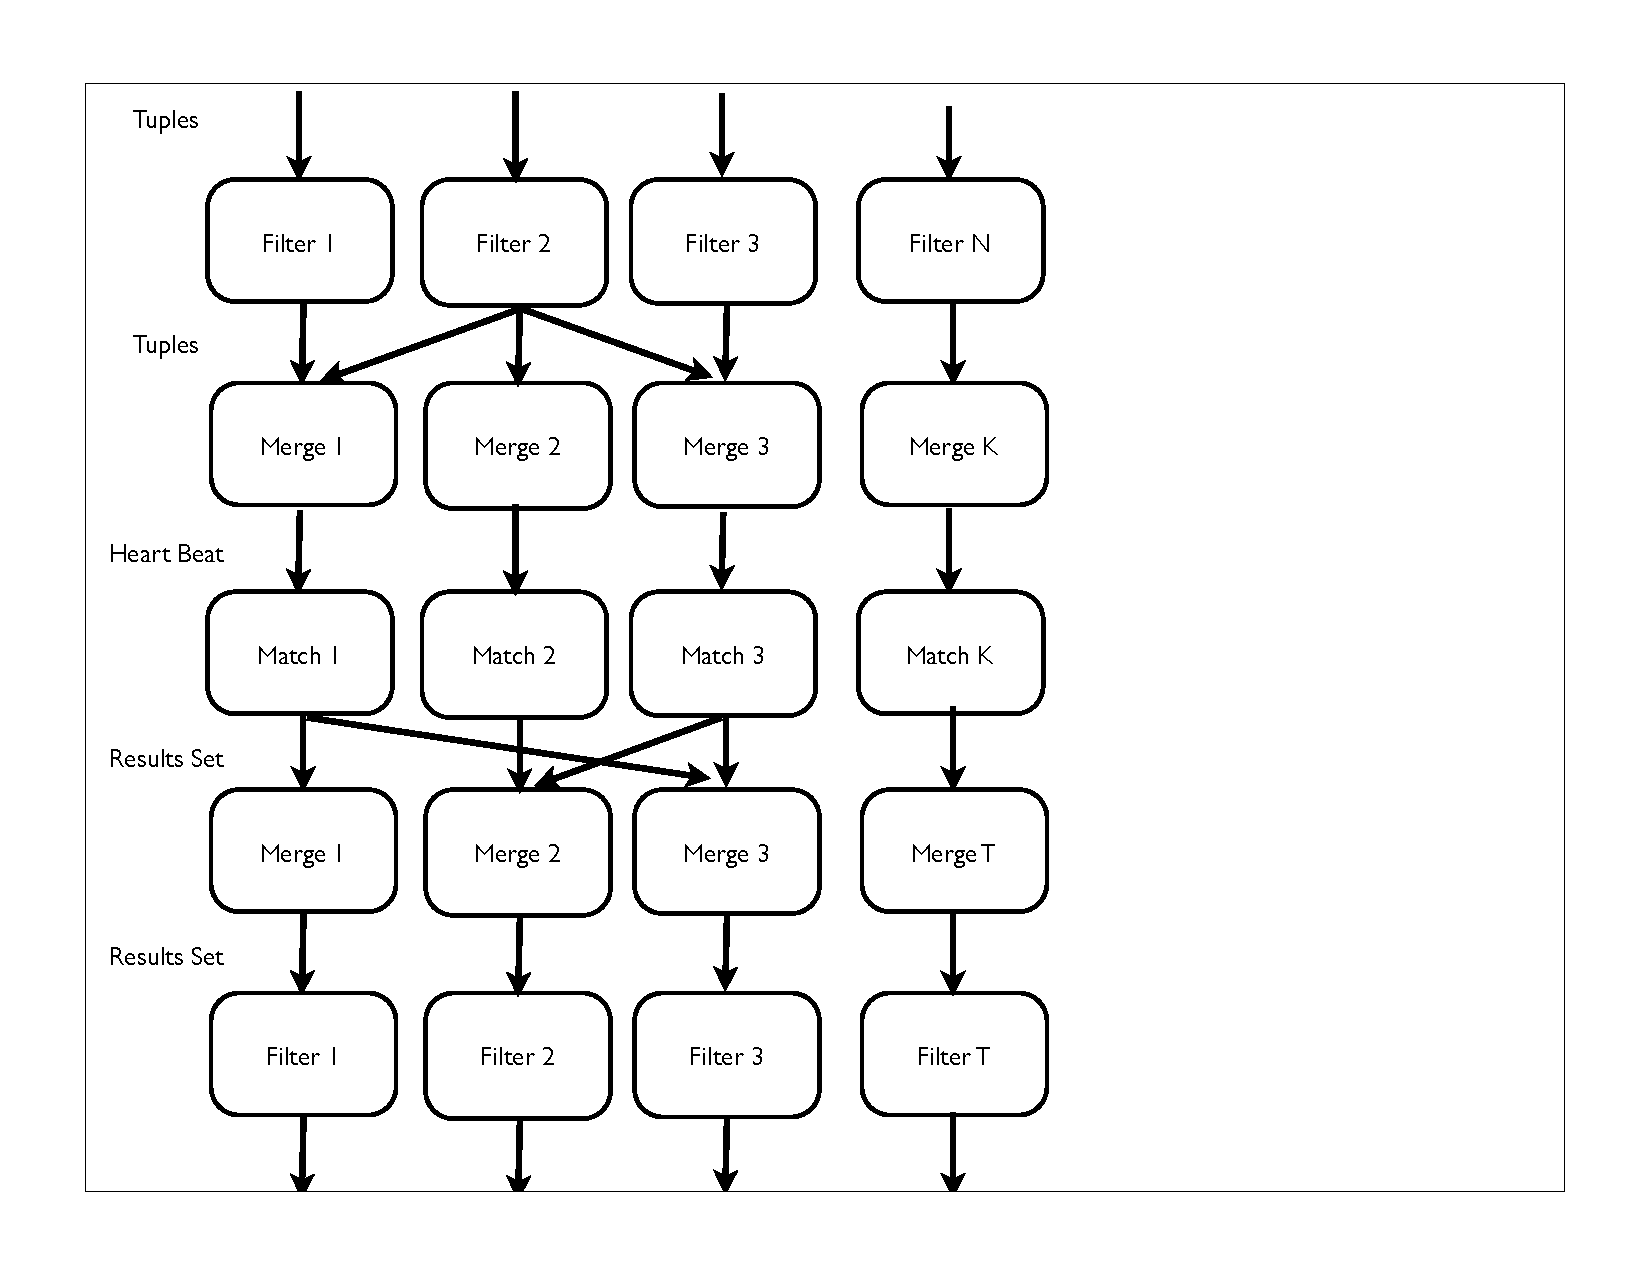
\includegraphics[width=4.50in]{figures/ExchangeFigure.pdf}
  \caption{Exchange Execution Path.}
  \label{fig:overview}
\end{figure}

Figure \ref{fig:overview} shows data execution paths and interactions between various components of the Exchange Server.

\section{Input Filter}

The goal of an input filter is to remove undesired tuples from input stream or to add tuples to the stream triggered by some input parameters.

The desired functionality is as follows:

\begin{program}
    \begin{verbatim}   
    while (input = getInputTuple)
    {
        if (match(input, conditions)
        {
            additionalInput=createAddInput(input);
        }
        if (match(input, bad_condition))
        {
            continue;
        }
        process(input, additionalInput);
    }
    \end{verbatim}
\caption{Input Filter Functionality.}
\end{program} 

Potential solution to this is to use generic SQL to filter incoming tuples. For instance the code to filter out tuples will look like:

\begin{program}
    \begin{verbatim}   
    select * 
    from input_stream
    where not(bad_condition)
    \end{verbatim}
\caption{SQL remove filter.}
\end{program}

Adding extra tuples can provide a bit trickier with SQL

\begin{program}
    \begin{verbatim}   
    select new_tuple
    from input_stream
    where (condition)
    \end{verbatim}
\caption{SQL add filter.}
\end{program}

\noindent The \emph{new\_tuple} fields will depend on some parameters of the condition as well as tuples coming from input stream.

Alternatively

\begin{quote}
A = LOAD STREAM {}``ABC'' USING LOADER() {[}AS SCHEMA{]};\\
B = FILTER A BY TIMESTAMP > X;\\
STREAM B INTO {}``XYZ'';
\end{quote}

The Exchange Server has two input streams. One stream is historical data from trades executed at some previous date. The second stream is additional trades coming from Trading Algorithms. The stream of updates coming from Trading Algorithms can be controlled by the user (At the moment we assume that users have complete control over trading algorithms). However, historical data can be dirty and incomplete. We want to give users control to restore or remove information impurities. For instance, data tuples, corresponding to orders that were completed, can be removed from the system since the Simulator will be able to create such a matching by itself. Also if we see a change in some order (the order was partially fulfilled) and we have no reference to such order in the order book, we would want to add such order to the book (the concerns for this operation are noted later).
Exchange Server Filtering can be implemented as follows:

\begin{program}
    \begin{verbatim}   
    while (input = getInputTuple())
    {
        messages;
        if (input.action == "F" || input.action == "E")
        {
            if (!checkTuple(relation, input.ID)
            {
                messages.add(getNewTuple(input));
            }
        }
        else
        {
            messages.add(input);
        }
        
        callMerging(messages);
    }
    \end{verbatim}
\caption{Add/Remove Filter for ESS.}
\end{program}

\noindent The \emph{getNewTuple(input)} function is undefined. Without additional information we do not know if an "S" or "B" tuple should be added as a result of an "F" or "E" input. This information could have been deduced from other messages, however there is no guarantee on the message order, making it impossible to tell which messages should be paired up. 

\section{Input Merging}

Often, once input is received, we would want to combine (join) two input streams or to impose future conditions (example windowing) on the input steam. Input Merging will allow users to specify those conditions and create additional relations form them.

\begin{program}
    \begin{verbatim}   
    getLock();
    while (input = getInput(sources))
    {
        if (conditions(input))
        {
            store (input);
        }
    }
    releaseLock();
    \end{verbatim}
\caption{Joining a set of sources and filtering on a set of conditions.}
\end{program}

In SQL we can represent this with 

\begin{program}
    \begin{verbatim}   
    select *
    from A
    where condition1
    UNION
    select *
    from B
    where condition2
    ...
    \end{verbatim}
\caption{Possible SQL Input Merging}
\end{program}

Alternatively 

\begin{quote}
A = LOAD STREAM {}``XYZ1'' USING LOADER();\\
B = LOAD STREAM {}``XYZ2'' USING LOADER1();\\
C = LOAD STREAM {}``XYZ3'' USING LOADER2();\\

D = UNION A, B, C;\\
E = SORT D BY TIMESTAMP;\\
STORE E INTO {}``OB'';
\end{quote}


A set of relations produced as a result of merging are matched in the Exchange Server. Merging provides a way to combine streams over which matching will be imposed. 

\subsection{Matching Policies}

The Exchange Simulator has eight matching policies:

\begin{enumerate}
    \item {\bf Only within, skip} matches orders coming from historical files only with historical files and orders coming from algorithms only with orders coming from algorithms.
    \item{\bf With anything} matches orders independent of origin, if a historic data match does not occur due to a match with a simulated order from an algorithm, a now unmatched historic order will be left in the order book. 
    \item{\bf With anything, drop} similar to a match with anything above but in this case a unmatched historic order will now be dropped.
    \item{\bf With Duplicate} if a historic order can be matched with an algorithmic order, create an artificial order equivalent to that of historic and match with this artificial order. Historic orders are only matched with historic orders. (looks for the first best match within both historic order and live orders). Each stock recorded in historic orders can be matched with only one simulated stock inquiry.  
    \item{\bf With Duplicate, live first} same as one before only first checks for a possible match with another live order, if one found do not look for historic match. 
    \item{\bf Drop with look ahead} similar to drop but historical matches are dropped only if they are close to the current match. (closeness can be measured by a sliding window of time or number of orders)
    \item{\bf Skip look back} similar to the first one, creates matches of historical with historical, and live with live orders within a sliding window of older orders. Orders older than sliding window can be matched with any new order regardless of it being historical or live.
\end{enumerate}

\noindent Here is how we can implement each one of them

A matching strategy \emph{Only within, skip} needs two relations: historical order-book and simulated order-book.

\begin{verbatim}   
function historicData(inputTuple)
{
    storeTuple(inputTuple, historicView);
    if (heartbeat())
    {
        callMatching();
    }
}

function simulatedData(inputTuple)
{
    storeTuple(inputTuple, simulatedView);
    if (heartbeat())
    {
        callMatching();
    }
}
\end{verbatim}

\noindent A matching strategy \emph{With anything} needs the following relation
\begin{verbatim}     
function allData(inputTuple)
{
   storeTuple(inputTuple, dataView);
   if (heartbeat())
   {
       callMatching();
   }
}
\end{verbatim}

\noindent \emph{With anything, drop}:
\begin{verbatim}     
function allData(inputTuple)
{
   if (unmatchedHistoric(inputTuple))
        return;
    
   storeTuple(inputTuple, dataView);
   if (heartbeat())
   {
       callMatching();
   }
}
\end{verbatim}

\noindent \emph{With Duplicate}: This strategy makes use of both historic and simulated data. Historic orders are matched only with other historic orders. Simulated orders can be matched with either a duplicate of historic orders or with other simulated orders. Similar to the \emph{skip} strategy from above we have two relations. This time a \emph{combinedView} relation will be a merged relation consisting of both historic and simulated tuples. A \emph{historicView} relation contains only historic tuples.

\begin{verbatim}   
function historicData(inputTuple)
{
    storeTuple(inputTuple, historicView);
    if (heartbeat())
    {
        callMatching();
    }
}

function combinedData(inputTuple)
{
    storeTuple(inputTuple, combinedView);
    if (heartbeat())
    {
        callMatching();
    }
}
\end{verbatim}

\noindent \emph{With Duplicate, live first} is the same as \emph{With Duplicate, once}. The matching function first tries to match simulated orders with simulated order in the \emph{combinedView} relation. When there is no matches between simulated order, the matching function will try to match historic tuples with simulated tuples.

\noindent \emph{Drop with look ahead} strategy is similar to \emph{With anything, drop}. It has a more complicated \emph{unmatchedHistoric} function.
\begin{verbatim}     
function allData(inputTuple)
{
   if (unmatchedHistoric(inputTuple, windowSize))
        return;
    
   storeTuple(inputTuple, dataView);
   if (heartbeat())
   {
       callMatching();
   }
}
\end{verbatim}

\noindent A \emph{Skip look back} matching strategy is similar to the skip strategy. It differs from it by moving tuples older than some "age" (measured in real time or in number of tuples seen) to a different, third relation.
\begin{verbatim}   
function historicData(inputTuple)
{
    storeTuple(inputTuple, historicView);
    oldTuples(historicView, windowConditions);
    storeTuples(oldTuples, oldTuplesView);
    if (heartbeat())
    {
        callMatching();
    }
}

function simulatedData(inputTuple)
{
    storeTuple(inputTuple, simulatedView);
    oldTuples(simulatedView, windowConditions);
    storeTuples(oldTuples, oldTuplesView);
    if (heartbeat())
    {
        callMatching();
    }
}
\end{verbatim}

\section{Experiment.}

Here we want to allow users to specify how to reduce or extract useful information from a simulation. A user sets specific conditions/rules on how to deal with each specific relation. 

\begin{program}
    \begin{verbatim}  
    if (heartbeat) 
        foreach (Relation r)
        {
            results = reduce(relation);
            output(results);
        }
    \end{verbatim}
\caption{Information Extraction.}
\end{program}

The \emph{reduce(relation)} function specifies what information is left, what tuples are still in the relation, and what tuples are not in the relation. The \emph{results} variable stores the consequences of the reduction. 

SQL does not have a very convenient way of specifying the above.

Exchange Server reduces relation by creating a matching between tuples in the relation.

\begin{program}
    \begin{verbatim}  
    foreach (Relation R)
    [R.sell, R.buy] = split(R);
    sort(R.sell, price, time);
    sort(R.buy, price, time);
    
    match=true;
    results;
    while (match)
    {
        topS=R.sell.top();
        topB=R.buy.top();
        [results, match] = tryMatching(topS. topB);
    }
    \end{verbatim}
\caption{Exchange Matching}
\end{program}


\section{Output Merging}

This is similar to input merging. The idea is to combine reduction results provided by a set of reduce functions from different relations into one stream. This can be done in a similar fashion. 

The Exchange Server outputs only one stream of updates. Thus, when matching occurs over a set of relations, they are combined into a single stream. 

%\emph{example?}

\section{Output Filtering} 

The idea behind filtering output is to impose extra conditions on output streams. This is similar to input filtering. 

In the case of the Exchange Server, we want to impose conditions on the output stream, such as price changes that are dependent on volume and time. 
\begin{program}
    \begin{verbatim}  
    while (tuple )
    {
        if (tuple.action = 'S' && tuple.volume > 1000)
            setOutputPriceIncrement(increment, duration);
    }
    \end{verbatim}
\caption{Exchange Output Filter.}
\end{program}

\section{Previous Discussions}

{\bf Determining Current Price} 

Current price is determined by a set of basic conditional rules. Time of the day OPENING, CONTINUOUS TRADING, CLOSING, AFTER HOURS, reference price and various trade stopping conditions together determine strategy for price resolution.

Here is a possible rule for current price determination

\begin{program}
    \begin{verbatim}    
    case POSITION:
        OPENING:
            case MATCHING_POLICY:
                BEST_VOLUME sPrice=bPrice=getBestVolume();
                AUCTION     sPrice=bPrice=performAcution();
                AVERAGE     sPrice=bPrice=getMean();
                ...
        TRADING:
            case MATCHING_POLICY:
                FIRST_IN_BOOK  sPrice=bPrice=existantTuple.price;
                AUCTION        sPrice=bPrice=performAcution();
                AVERAGE        sPrice=bPrice=getMean();
                LAST_COME      sPrice=bPrice=newTuple.price;
                BEST_REMAINING sPrice=bPrice=getNextTuple.price;
                DOUBLE_AUCTION some form of equialibrium.
                ...       
        CLOSING:
            case MATCHING_POLICY:
                BEST_VOLUME sPrice=bPrice=getBestVolume();
                AUCTION     sPrice=bPrice=performAcution();
                AVERAGE     sPrice=bPrice=getMean();
                ...
        AFTER_HOURS:
            case MATCHING_POLICY:
                BEST_VOLUME sPrice=bPrice=getBestVolume();
                AUCTION     sPrice=bPrice=performAcution();
                AVERAGE     sPrice=bPrice=getMean();
                ...
    \end{verbatim}
\caption{Price Strategy. }
\end{program}

The more complete matching rules are in Swiss Stock Exchange paper.
\\
\\
{\bf Execution Loop Variations}

\begin{description}
    \item[Update Driven Execution] every data update trigers an action from a server. On an order placement (Bid/Ask order) server attempts to match it with an order in an order book. On delete an order is removed from the book (if present).
    \item[Batch Driven Execution] Data updates are collected and actions are performed in a batch over s set of updates. Orders are not executed during the collection phase, some basic statistics about collected orders can be published. When conditions are satisfied (either time, amount or the combination of the two conditions) orders are executed (in the end of tick) and a set of actions is performed. (A possible variation is to batch only inserts bids/asks and let other updates be executed immediately.)
    \item[Other ideas] ???
\end{description}

Both approaches have pros and cons. Update execution creates fast FIFO (price, time) order processing with competitive price. Batch execution though slower in response time is capable of supporting double auction matching and best volume matching, which first approach cannot execute. 
\\
\\
{\bf Order Matching} 
\\
There are several possible scenarios to integrate orders coming from simulated algorithms (live) to orders coming from historical (historic) data files.
\\
\noindent Matching Policies:
\begin{enumerate}
    \item {\bf Only within, skip} matches orders coming from historical files only with historical files and orders coming from algorithms only with orders coming from algorithms.
    \item{\bf With anything} matches orders independent of origin, if a historic data match does not occur due to a match with a live order from an algorithm, a now unmatched historic order will be left in the order book. 
    \item{\bf With anything, drop} similar to a match with anything above but in this case a unmatched historic order will now be dropped. 
    \item{\bf With Duplicate} if a historic order can be matched with algorithmic order, create an artificial order equivalent to that of historic and match with it. Historic orders are only matched with historic orders. (looks for the first best match within both historic order and live orders)
    \item{\bf With Duplicate, once} same as above only it keep track of, which historic orders where matched with live orders so not to match them more than once. 
    \item{\bf With Duplicate, live first} same as one before only first checks for a possible match with another live order, if one found do not look for historic match. 
    \item{\bf Drop with look ahead} similar to drop but historical matches are dropped only if they are close to the current match. (closeness can be measured by a sliding window of time or number of orders)
    \item{\bf Skip look back} similar to the first one, creates matches of historical with historical, and live with live orders within a sliding window of older orders. Orders older than sliding window can be matched with any new order regardless of it being historical or live.
\end{enumerate}

Neither of the above matching rules is perfect. Here are some of their drawbacks:

Numbers 1 and 8 can create an order book imbalance where current price for historical orders does not reflect the changed reality of added live orders. Number 8 is an attempt to correct this problem. Rules 2-7 do not reflect the actual historical behavior. 
\\
\\
{\bf First draft of scripting language}
\\
These parameter settings can be unified in:
\begin{program}
    \begin{verbatim}
    select execution with execution_params
    set pricing_model with pricing_params
    groupby matching_strategy with matching_params
    \end{verbatim}
    \caption{Script}
\end{program}  

Where \underline{execution} is either batch matching or a single tuple match. \underline{pricing model} is a way to determine current price and \underline{matching strategy} is a best way to match historic and algorithmic orders.
\\
\\
{\bf Second draft of scripting language}
\\
Our basic premise is that matching between order occurs within an order book. An order book contain live and historic order can be though of as a relation. A select query over that relation can be though as a filter for tuples in that relation.

For instance, query 

\begin{program}
    \begin{verbatim}
    select * as Live_View
    from   all_tuples_relation T
    where T.place == live_tuple
    \end{verbatim}
    \caption{Selection filter}
\end{program}

\noindent creates an order book over updates from Trading Algorithms. Syntax for a filters is a subset of SQL. 

SQL inspired matching language can have the following form:

\begin{program}
    \begin{verbatim}
    matching E, F as Results
    from Live_View
    with avg_price
    using batching with ticker
    \end{verbatim}
    \caption{Matchings Example}
\end{program}

The matching language syntax is:
\\
\\
Matching \emph{type}, ... as \emph{place} \\
from [\emph{then} $\vert$ \emph{combined}] \emph{Filters} \\
with \emph{price\_strategy} $\vert$ (\emph{Time}, \emph{price\_strategy}), ...\\
using \emph{execution\_mode} [with \emph{execution\_parameters}]



\end{document}

extra coments

